\chapter{Avaliação} \label{ch:evaluation}

Este Capítulo apresenta resultados comparativos da solução desenvolvida com a 
aplicação original. A Seção \ref{sect:methodology} apresenta os detalhes da 
avaliação e a Seção \ref{sect:results} disserta sobre os resultados.


\section{Metodologia de Avaliação} \label{sect:methodology}

Os experimentos foram realizados no Parque Computacional de Alto 
Desempenho (PCAD) da UFRGS. Eles ocorreram nos nós de computação draco, sua 
configuração é mostrada na Tabela \ref{tab:draco_config}. Foram realizados 
testes em uma máquina, com a implementação original da aplicação e em múltiplas 
máquinas, utilizando a implementação modificada.

\begin{table}[H]
\centering
\begin{tabular}{l l} \toprule
\textbf{Parâmetro}  &  \textbf{Configuração} \\ 
\midrule
Processador     & 2 x Intel Xeon E5-2630 (Q1'12) Sandy Bridge, 2,5 GHz  
\\
Número de Núcleos    & 16 núcleos (8 por CPU)  \\
Memória       & 64 GB DDR3 RAM   \\
\end{tabular}
\caption{Configurações dos nós draco.}
\label{tab:draco_config}
\end{table}


Nos testes distribuídos, inicialmente executamos o Hadoop para copiar as 
entradas para o HDFS. Um dos nós era responsável por executar o \emph{namenode}, 
e também executava uma instância de \emph{datanode}. Os demais executavam apenas 
instâncias de \emph{datanodes}.

O gerenciador de cluster utilizado foi o do próprio Spark ao invés do YARN. 
Essa decisão foi tomada durante os testes pois seus logs mostraram 
informações mais claras sobre o que estava ocorrendo. A instânciação dele foi 
similar àquela utilizada no Hadoop, onde um nó executou como mestre e 
trabalhador enquanto os demais executaram apenas como trabalhadores. Além 
disso, o mesmo nó que executou o \emph{namenode} Hadoop foi o que executou o 
mestre Spark.

Realizamos testes com um nó, utilizando a aplicação original, dois e três nós, 
utilizando a aplicação modificada. Cada teste foi executado múltiplas vezes 
para garantir a confiabilidade de seus resultados. Nos experimentos, nenhuma 
configuração do Spark foi definida, utilizou-se os valores padrão que a engine 
definiu.


\section{Experimentos e Resultados} \label{sect:results}

A carga de trabalho dos experimentos já no formato CSV (entrada para a fase de 
pré-processamento no StarVZ), tinha um somatório de 12 GB. Ela consiste em 
rastros de execução de uma aplicação cholesky, e foi escolhida pois era a maior
entrada que tínhamos no momento. O tamanho de cada um dos arquivos pode ser 
visualizado na Tabela \ref{tab:input_sz}.

\begin{table}[H]
\centering
\begin{tabular}{l c} \toprule
\textbf{Arquivo}  &  \textbf{Tamanho} \\ 
\midrule
state.csv	& 6.8 GB \\
variables.csv  	& 2.5 GB \\
link.csv       	& 304 MB \\
dag.csv        	& 270 MB \\
entities.csv	& 73 KB \\
events.csv	& 1.8 GB \\
\textbf{Total}  & 12 GB  \\
\end{tabular}
\caption{Detalhamento da carga de trabalho.}
\label{tab:input_sz}
\end{table}

Durante a implementação, optou-se por manter o processamento do arquivo entities 
no formato sequencial pois esse arquivo armazena apenas informações de 
plataforma e por isso, costuma não passar da ordem de tamanho de KB. Podemos 
observar que isso se confirma nessa carga de trabalho.

Nas execuções distribuídas, o Spark alocou diferentes configurações por nó, 
como pode ser visualizado na Tabela \ref{tab:spark_def_config}. É importante 
salientar que a definição dessas configurações foram decididos pela engine, 
pois não houve parametrização.


\begin{table}[H]
\centering
\begin{tabular}{c c c c} \toprule
\textbf{Número de nós}  &  \textbf{Executores por Nó} & \textbf{Cores por 
Executor} & \textbf{Memória por Executor} \\ 
\midrule
2	& 16 & 2 & 3 GB\\
3	& 15 & 2 & 4 GB\\
\end{tabular}
\caption{Ambiente instânciado pelo Spark.}
\label{tab:spark_def_config}
\end{table}

Tratando-se dos resultados, foram executadas 30 repetições dos testes, mas para 
o cálculo da média e desvio padrão dos testes com dois e três nós, utilizou-se 
apenas 29 resultados pois uma repetição apresentou problemas de execução. Como 
isso foi um caso isolado, sua causa não foi investigada.

A Figura \ref{fig:total_full} mostra a média do tempo total de execução dos 
experimentos e o desvio padrão no topo da barra. A execução original, de forma 
sequencial, levou em média 1489,02 segundos para completar o processamento. Já 
as execuções com a aplicação adaptada para utilizar o Spark, com dois nós levou 
461,99 segundos e com três, 385,44 segundos. Isso consiste em um \emph{speedup} 
de respectivamente 3,22x e 3,86x em relação ao original.


\begin{figure}[H]
\centerline{
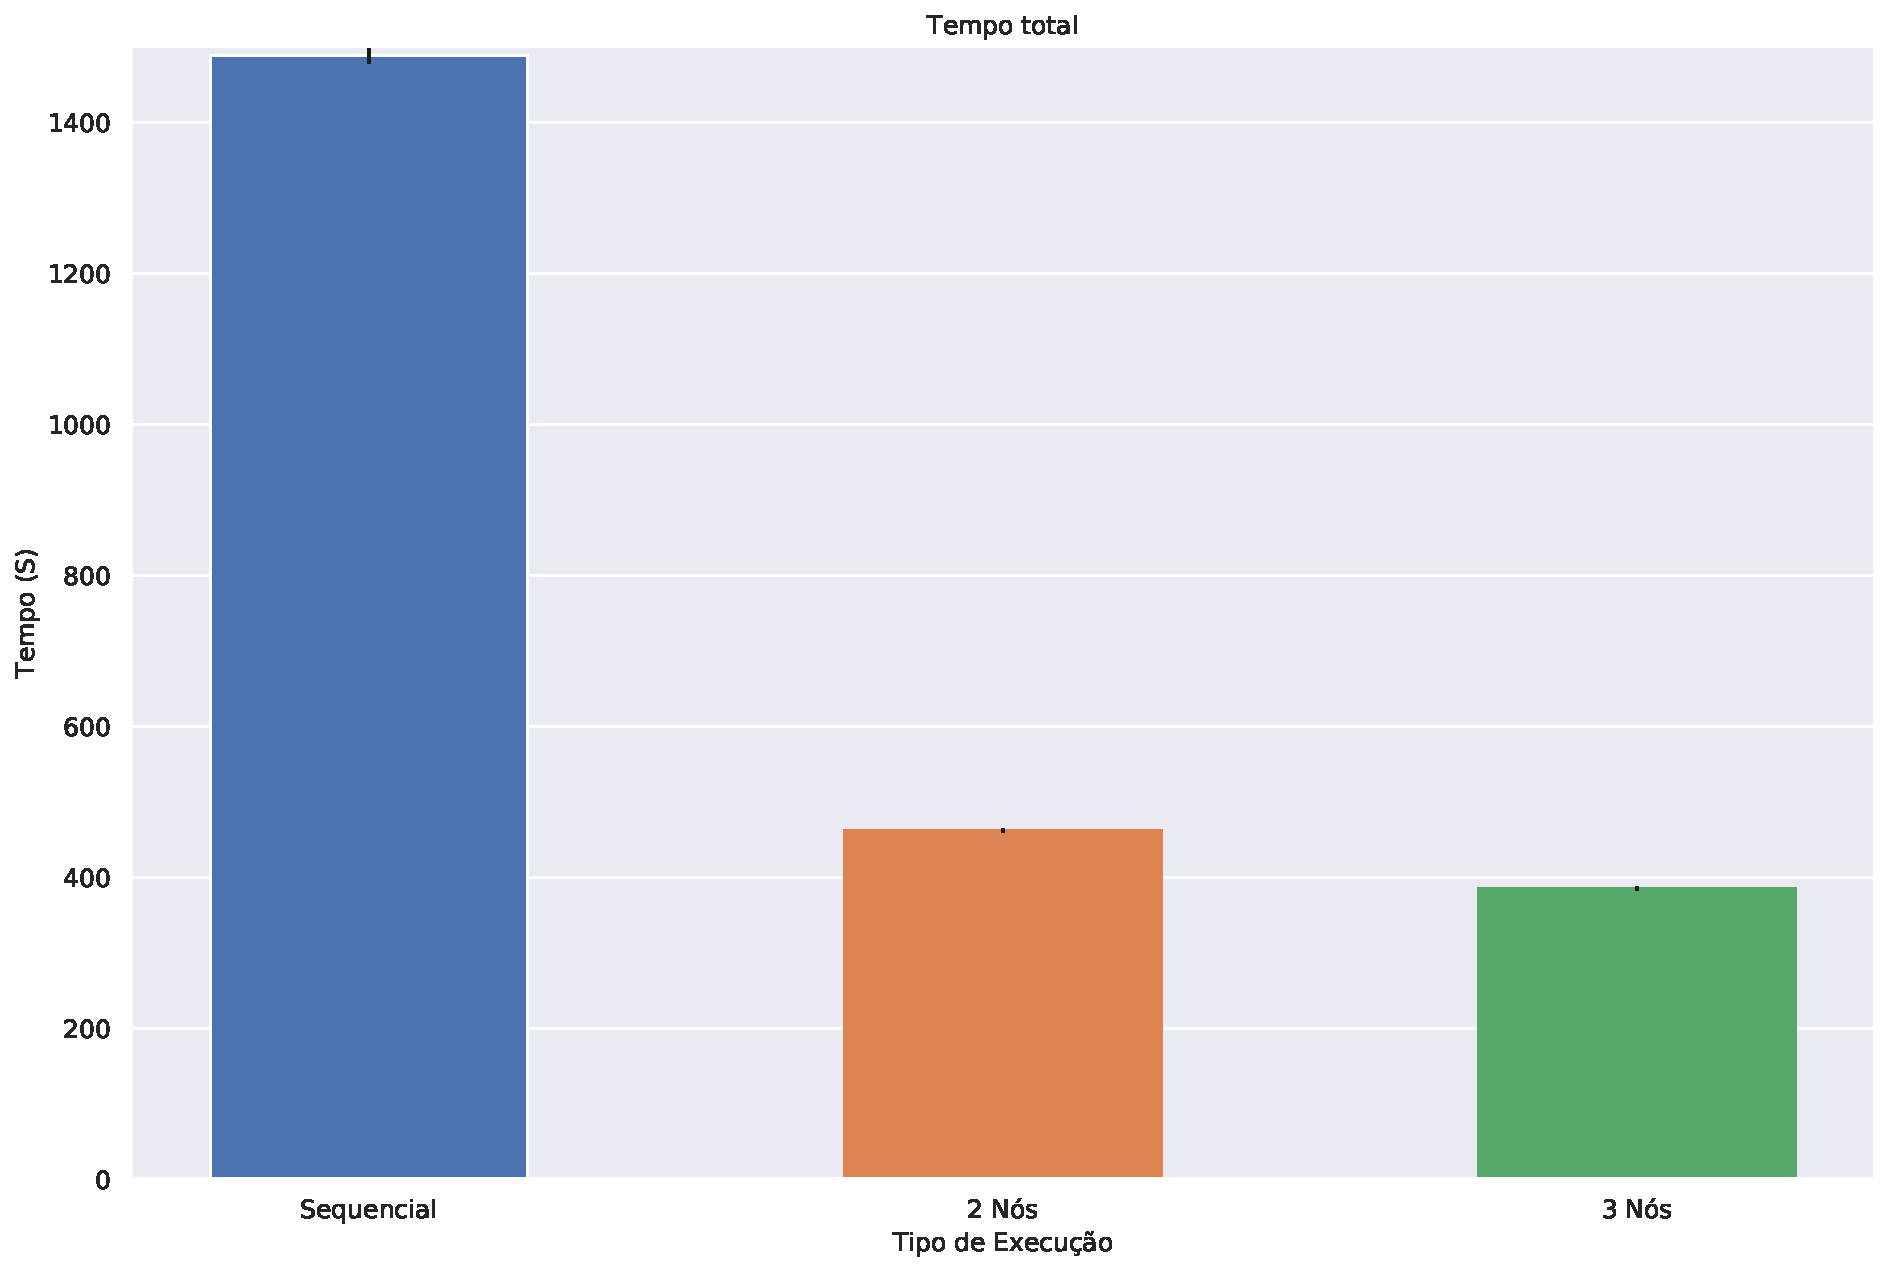
\includegraphics[width=0.9\textwidth]{./img/total.pdf}}
 \caption{Tempo total de execução da aplicação.}
 \label{fig:total_full}
\end{figure}

Segmentamos a análise por etapa exibida na Figura \ref{fig:spark-starvz-flow}, 
seus tempos de execução podem ser visualizados na Figura \ref{fig:total_step}. 
Fica claro que o processamento dominante em todos os tipos de execução é o de 
State. Todavia, comparando os experimentos distribuídos com o sequencial, 
concluímos que sua dominância não é relacionada ao seu tamanho mas sim as 
manipulações realizadas com ele.

\begin{figure}[H]
\centerline{
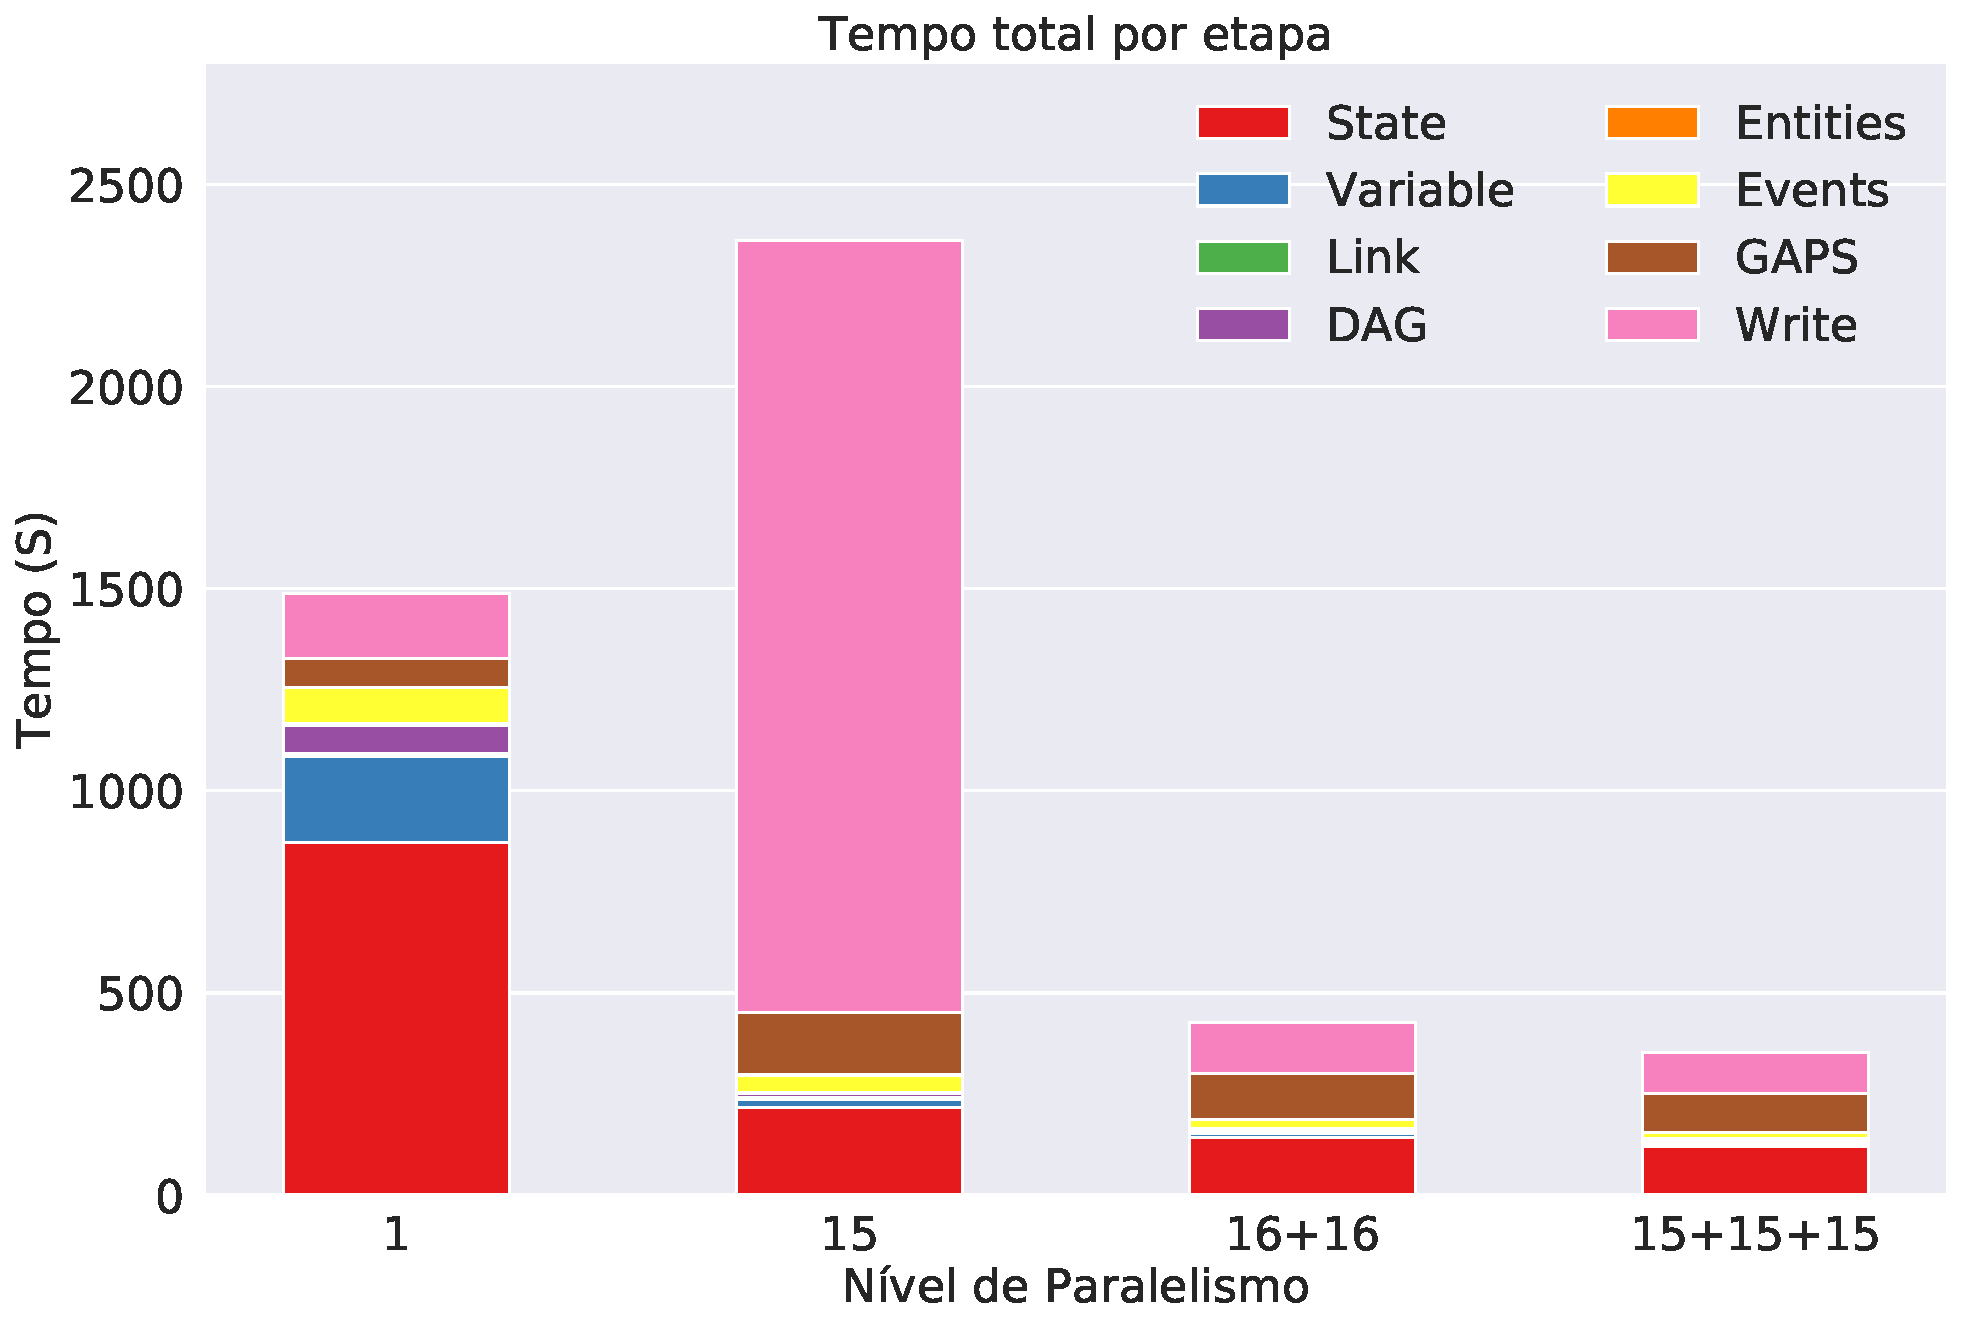
\includegraphics[width=0.9\textwidth]{./img/total_step.pdf}}
 \caption{Tempos de execução segmentados por etapas.}
 \label{fig:total_step}
\end{figure}

Analisando o processamento de variables, o segundo maior arquivo da carga de 
trabalho, na execução sequencial é o segundo mais custoso levando em média 
210,77 segundos. Já na distribuída seu tempo cai para 8,50 segundos com 2 nós e 
7,50 com três, representando um \emph{speedup} de respectivamente 24,79x e 
28,10x.

Ao comparar-se as manipulações realizadas entre esses dois arquivos, em 
variables são realizadas filtragens e manipulações na própria tabela, enquanto 
states possui algumas junções de tabelas. Também há a definição de uma variável 
que exige que seja executada uma operação \texttt{sdf\_collect}, que ao ser 
executada em uma tabela Spark, trás os dados para uma tabela local. Portanto é 
possível haver pontos de otimização dentro dessa função que levem a 
\emph{speedups} ainda melhores.

O processamento de entities fora mantido na forma sequencial devido ao seu 
tamanho ser na ordem de KB. Seu tempo de processamento tem um valor irrisório 
a ponto de ser difícil de observar no gráfico. Em média, para a execução com 
um nó ele levou 3,07 segundos, já com dois e três nós foram respectivamente 
2,29 segundos e 2,30 segundos. Portanto, nossa decisão teve pouco impacto no 
resultado final, o que era o objetivo já que sua constribuição para o tempo 
total da aplicação é tão pequeno e o custo para processá-lo de forma 
distribuída prejudicaria o resultado.

GAPS fora levantado durante a implementação como um ponto de atenção, devido ao 
seu tempo ter aumentado considerável em experimentos locais. 

















% \begin{figure}[ht]
% \centerline{
% 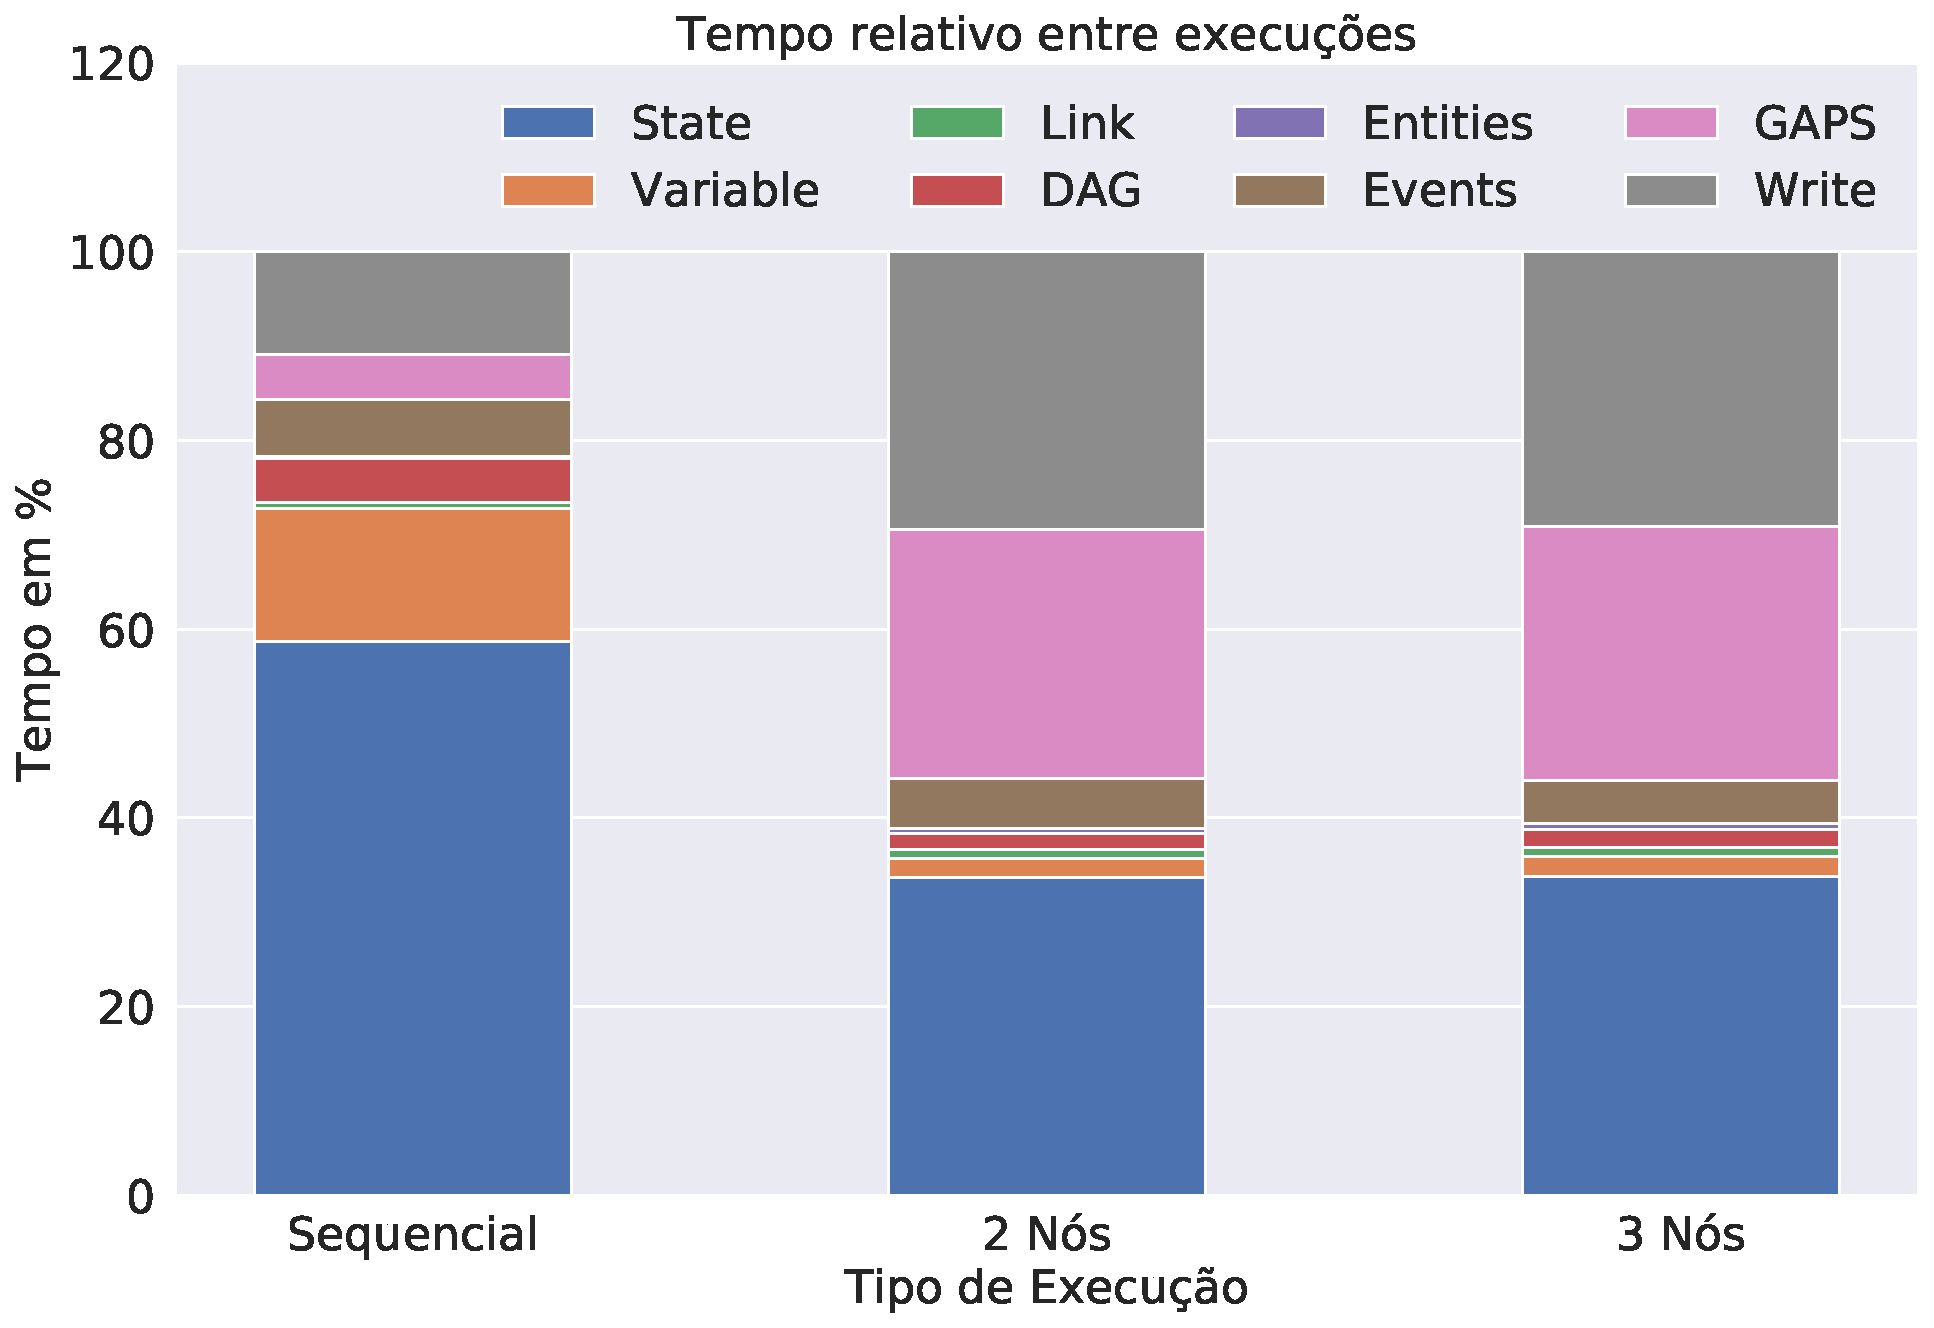
\includegraphics[width=1\textwidth]{./img/total_relative.pdf}}
%  \caption{Tempos de execução segmentados por etapas.}
%  \label{fig:total_step}
% \end{figure}


